%Ab Hier kommen die Einstellungen für das NEUE APQ-TUD_Design!!!
\documentclass[
class=book,
accentcolor=1b,
custommargins=geometry,
fontsize=11pt,
thesis={type=Versuchsanleitung},
ruledheaders=all,
headline=false,
instbox=false,
marginpar=false,
title=small,
ignore-missing-data=true,
twoside=false,
pdfa=false % Problem mit Paket pdfx
]{apqpub} 

% % % % % % % %
%Pakete
\usepackage{cancel}
\usepackage{float}
\usepackage{subfig}
\usepackage{amsmath,amsthm,amssymb,dsfont}
\usepackage{mathtools}
\usepackage{mathrsfs}
\usepackage{enumerate}
\usepackage{isotope}
\usepackage[ngerman]{babel}
\usepackage[utf8]{inputenc}
\usepackage{nicefrac}
\usepackage{upgreek}
\usepackage[section]{placeins}
\usepackage{braket}


\usepackage[backend=bibtex, sorting=none, style=numeric-comp, defernumbers]{biblatex}
\addbibresource{mybib}

%\usepackage{multibib}
%\newcites{q}{Quellen}
%\newcites{erg}{Ergänzende Literatur}
%\newcites{wes}{Wesentliche Literatur}


\usepackage{siunitx}
\sisetup{
  locale = DE ,
  per-mode = fraction,
%  per-mode = symbol,
  math-micro = \upmu,
  text-micro = µ,
  separate-uncertainty = false,
}

\usepackage{geometry}
\geometry{
	reset,
	a4paper,
	top=20mm,
	bottom=25mm,
	inner=31mm,%7mm Bindekorrektur sind jetzt
	outer=24mm,%der neue Standard im APQ-Design!
	includefoot,
	includehead,
	footskip=10mm,
	nomarginpar
}

\usepackage{hyperref} % Immer als letztes laden
\def\UrlFont{\normalfont}
% % % % % % % %
%Weitere Änderungen
\DeclareOldFontCommand{\bf}{\normalfont\bfseries}{\mathbf}
%\renewcommand{\it}{\textit}
\RedeclareSectionCommand[afterskip=\baselineskip]{chapter}
\newcommand\todo[1]{\textcolor{red}{#1}}
\parindent 0pt
\addtokomafont{caption}{\rmfamily\small}
\addtokomafont{captionlabel}{\accentfont}



\addTitleBoxLogo*{\makebox[\linewidth][l]{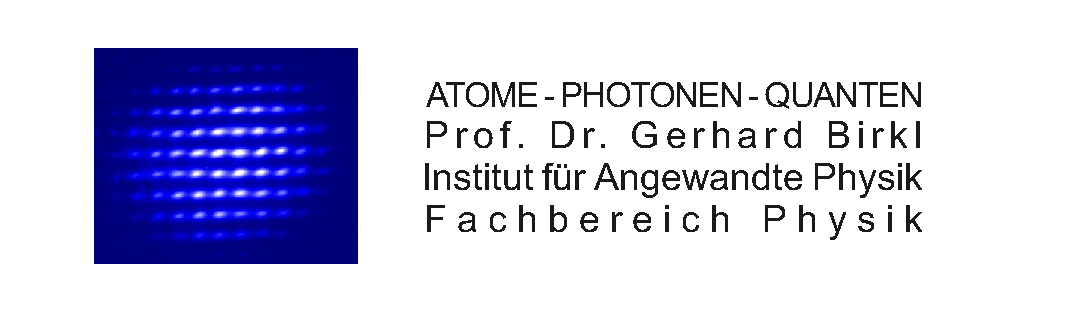
\includegraphics[width=55mm]{titel_apq-logo_1.pdf}}}

\graphicspath{{C:/Users/Max_Mustermann/Uni/Master/Masterarbeit/Results/}}%Möglichkeit einen generischen Pfad zu Abbildungen anzugeben.

%\lowertitleback{Textblock auf der Rückseite des Titelblattes. Enthält in der Regel Informationen über das Titelbild.}

\begin{document}
\renewcommand*{\figurename}{Abb.}
%\renewcommand*{\figurename}{Fig.} %Für englische Dokumente auskommentieren
\renewcommand*{\tablename}{Tab.}
	\titleimage{\includegraphics[width=\textwidth]{graphics/title_okt23_2.png}}
	
	%%% Problem mit pdfx-Paket Start
	%\Metadata{
	%	title= Titel der Thesis, %% TUDaThesis -- Template für Abschlussarbeiten im CD der TU Darmstadt,
	%	author=Max Mustermann
	%}
	%%% Problem mit pdfx-Paket Ende
	
	%%%% Für den Titel sind 3 Zeilen vorgesehen.
	%%%% Hat der Titel nur zwei Zeilen, ist ein Zeillenumbruch (\\) einzufügen, um den Titel oben bündig zu positionieren
	%%%% Ist der Titel einzeilig sind zwei Freizeilen (\\ \ \\) anzuhängen.
	%%%% Ludwig Lind 03.02.2021
	\title{Fortgeschrittenenpraktikum \\ Abteilung A \\ 4.18 Mikro- und Fourieroptik}
	\subtitle{Micro and Fourier Optics}
	%\author[Max Mustermann]{Max Mustermann}%optionales Argument ist die Signatur,
	%\birthplace{Geburtsort}%Geburtsort, bei Dissertationen zwingend notwendig
	%\reviewer{Prof. Dr. Gerhard Birkl \and 2ter Gutachter}%Gutachter
	
	%Diese Felder erden untereinander auf der Titelseite platziert.
	%\department ist eine notwendige Angabe, siehe auch dem Abschnitt `Abweichung von den Vorgaben für die Titelseite'
	%\department{Fachbereich Physik} % Das Kürzel wird automatisch ersetzt und als Studienfach gewählt, siehe Liste der Kürzel im Dokument.
	%\institute{Institut für angewandte Physik}
	%\group{Atome-Photonen-Quanten}
	
	\submissiondate{\today}
	\examdate{\today} %\today
	\thesisdate{Stand Oktober 2023}
	
	%	\tuprints{urn=1234,printid=12345}
	%	\dedication{Für alle, die \TeX{} nutzen.}
	
	\maketitle
	\frontmatter
	
	%Füge in Abgaben mit twoside=false (z.B. Proposal) trotzdem titleback ein
%	\makeatletter
%	\if@twoside
%	\else%
%	\begingroup
%	\begin{minipage}[t]{\textwidth}
%		\@uppertitleback
%	\end{minipage}\par
%	\vfill
%	\begin{minipage}[b]{\textwidth}
%		\@lowertitleback
%	\end{minipage}\par
%	\@thanks\let\@thanks\@empty
%	\endgroup
%	\clearpage
%	\fi%
%	\makeatother
	 
%	\abstract{Inhaltliche Zusammenfassung der Thesis. Pflicht bei Masterarbeiten.}
	\tableofcontents
	
	\mainmatter
	\setcounter{page}{1}
	\chapter{Physikalische Grundlagen}
	\section{Gaußstrahl}
Das von Lasern ausgestrahlte Licht lässt sich häufig als sogenannter Gaußstrahl beschreiben.

In Abbildung \ref{fig:gauss} ist der Verlauf eines Gaußstrahls visualisiert.
\begin{figure}[H]
\centering
	\includegraphics[width=0.9\textwidth]
	{graphics/strahl_gauss.png}
\caption{Profil eines propagierenden Gaußstrahls \protect\cite{gauss}.}
\label{fig:gauss}
\end{figure}
Gaußstrahlen zeichnen sich dadurch aus, dass die Amplitude des elektromagnetischen Feldes im Raum durch 
\begin{align*}
E \left (r, z\right) = E_0 \frac{w_0}{w\left( z \right)} 
\exp \left( - \left( \frac{r}{w \left( z \right)} \right)^2 \right) 
A \left( r, z \right)
\end{align*}
beschrieben wird \cite[S. 50 -- 52]{Meschede}.
Dabei ist $z$ die Raumkoordinate in Propagationsrichtung, während $r$ die Radialkomponente in der zur $z$-Achse senkrechten Ebene beschreibt.
Die Verteilung ist offensichtlich radialsymmetrisch, da keine Abhängigkeit vom azimuthalen Winkel vorliegt.
Der Wert $E_0$ gibt die maximale elektrische Feldstärke an.
Mit $w_0$ wird der Strahlradius an der schmalsten Stelle des Gaußstrahls bezeichnet.
Für diesen Wert ist auch der Begriff Strahltaille gebräuchlich. 
Der Strahlradius ist allgemein als der Radius definiert, bei dem die elektrische Feldstärke auf den Faktor $\frac{1}{\mathrm{e}}$ des maximalen Werts abgefallen ist.
Die Funktion 
\begin{align*}
w \left( z \right) \coloneqq w_0 \sqrt{1+\left(\frac{z}{z_R}\right)^2}
\end{align*}
beschreibt den Strahlradius in Abhängigkeit von der $z$-Position.
Die Rayleighlänge $z_R$ ist dabei über $z_R \coloneqq \frac{\pi w_0^2}{\lambda}$ mit der Wellenlänge $\lambda$ verknüpft.
Sie beschreibt nach welcher Weglänge der Strahlradius auf $\sqrt{2} w_0$ angewachsen ist und gibt somit eine Abschätzung an, für welche Abstände näherungsweise von kollimierten Strahlen ausgegangen werden kann.
Der Faktor $A\left( r, z \right)$ trägt nur Phaseninformationen und soll hier nicht eingehend diskutiert werden, da er bei der Bestimmung der Intensität zu $1$ wird.

Für die Intensität eines Gaußstrahls gilt
\begin{align*}
I \left (r, z\right) = I_0 (z)
\exp \left( - 2 \left( \frac{r}{w \left( z \right)} \right)^2 \right) ,
\end{align*}
wobei $I_0 \left(z\right)$ die maximale Intensität in der jeweiligen Ebene bezeichnet.

Durchläuft ein Gaußstrahl eine Linse, so verändern sich die Strahltaille sowie die Position der Fokalebene.

Liegt der Fokus eines Gaußstrahls mit Strahltaille $w$ im Abstand $s$ vor einer Linse der Brennweite $f$, so gilt für den Strahl hinter der Linse

\begin{subequations}
\begin{align*}
s' &= f + \frac{f^2 \left( s - f \right)}{\left( s - f \right)^2 + z_R^2}  \\
\label{eq:gausswaist}
\text{und} \quad w' &= w f \sqrt{\frac{1}{\left(s-f\right)^2+z_R^2}}.
\end{align*}
\end{subequations}
Dabei bezeichnet $z_R$ die Rayleighlänge des Strahls vor der Linse.
Die Strahltaille kann also über Linsensysteme maßgeblich verändert werden.

	\section{Räumliche Modulation von Lichtfeldern}
Um möglichst beliebige elektromagnetische Felder zu erzeugen sind räumliche Lichtmodulatoren (engl. Spatial Light Modulators; kurz.: SLM) eine gute Wahl.
Hier sollen zwei im Laboralltag anwendbare Arten von SLM vorgestellt werden. 
	\subsection{Digitale Mikrospiegeleinheit}
Versatile Werkzeuge zur Intensitätsmodulation von Lichtfeldern stellen digitale Mikrospiegeleinheiten (engl.: Digital Micro-Mirror Devices; kurz: DMD) dar.
Der Vorteil dieser besteht in der einfachen Ansteuerung über einen Computer und der Variabilität der anzeigbaren Strukturen.
Die Nutzung der DMD hat sich in der experimentellen Praxis als praktisch erwiesen.
Verwendet wird im Versuch das Modell DLP3000 LightCrafter Evaluation Module von Texas Instruments \cite{manual:DMD}.
\begin{figure}
\centering
    \includegraphics[width=0.75\textwidth]
    {graphics/dmd_axis.png}
\caption{Schematische Darstellung der Anordnung der Einzelspiegel auf dem DMD \protect\cite{manual:DMD}.}
\label{fig:dmdanordnung}
\end{figure}
Die Oberfläche des DMD ist mit $\SI{415872}{}$ quadratischen Einzelspiegeln besetzt, die entsprechend Abbildung \ref{fig:dmdanordnung} diagonal angeordnet sind.
Die gesamte Spiegeleinheit hat eine Breite von $\SI{6.6}{\milli \metre}$ und eine Höhe von $\SI{3.7}{\milli \metre}$.
Die Einzelspiegel haben einen Abstand  von $\SI{7.637}{\micro\metre}$ und können in der Horizontalen, also um die vertikal orientierte Diagonale, gegenüber der normalen Position um $\pm \SI{12}{^\circ}$ verkippt werden.
Im Betrieb können nur diese beiden Positionen eingestellt werden.
Die Ansteuerung erfolgt also mit einer Bittiefe von $1$.
Die Spiegel können dann als \glqq schwarze\grqq{} oder \glqq weiße\grqq{} Pixel verwendet werden, in dem Sinne, dass bei schwarzen Pixeln das Licht so wegreflektiert wird, dass es verloren geht, während es bei weißen Pixeln in den weiteren optischen Aufbau gelegt wird.
Die Belegung ist dabei davon abhängig, aus welchem Winkel der DMD beleuchtet und aus welcher Richtung er beobachtet wird.
Für die meisten optischen Aufbauten ist es am geeignetsten, wenn der auslaufende Strahl senkrecht zur Oberfläche des DMD gerichtet ist.
Da die Abstände der Einzelspiegel mit $g = \SI{7.637}{\micro\metre}$ lediglich wenige Vielfache der im Versuch verwendeten Wellenlänge $\lambda = \SI{637 \pm 3}{\nano\metre}$ betragen, stellt das Mikrospiegelregister ein Blaze-Reflexionsgitter dar \cite[S. 947 -- 954]{Hecht}.
Dessen zweidimensionale Ordnung $\left( 3 , 3 \right)$ entspricht wegen der diagonalen Anordnung der Spiegel und der damit einhergehenden Drehung der Hauptachsen einer Ablenkung in horizontaler Richtung um $\sqrt{2} \cdot \arcsin \!\left(3 \cdot \frac{\SI{637 \pm 3}{\nano\metre}}{\SI{7.64}{\micro\metre}} \right) = \SI{20.5 \pm 0.1}{^\circ}$.
Da ein einzelner Mikrospiegel aufgrund der horizontalen Verkippung um $\SI{12}{^\circ}$ das Licht unter einem Beleuchtungswinkel von $\SI{24}{^\circ}$ wie gewünscht ablenken würde, ist die Ordnung $\left( 3 , 3 \right)$ des reflektierten zweidimensionalen Interferenzmusters die dazu nächstgelegene.
Sie trägt also einen Großteil der Leistung und wird deshalb in diesem Versuch verwendet.

	\subsection{Flüssigkristallanzeigen}
Auch Flüssigkristallanzeigen stellen eine gute Option als räumliche Lichtmodulatoren dar.
Mit ihnen lässt sich die Polarisation lokal manipulieren.
Dies bewirkt auch einen Phasenversatz, der als Grundlage des SLM dienen kann.
Weiterhin können LCD in Kombination mit polarisationsfilternder Optik als Intensitätsmodulatoren verwendet werden.
In dieser Konfiguration findet ein LCD in diesem Versuch Anwendung.

Konkret kommt die LCD-Einheit eines kommerziellen Beamers (Sharp PG-C30XE) zum Einsatz.
Diese hat eine Breite von $\SI{18.5}{\milli \metre}$ und eine Höhe von $\SI{13.9}{\milli \metre}$ \cite{manual:Sharp}. 
Insgesamt besteht die LCD-Einheit aus $\SI{786 432}{}$ Pixeln, die sich auf das Bildformat $\SI{1024}{} \times \SI{768}{}$ des Beamers verteilen. 

\section{Kamera}
Im Laufe des Versuchs findet eine Kamera bei der Aufnahme von Lichtfeldern Anwendung.
Konkret handelt es sich um das Modell Dragonfly2 DR2-BW aus dem Hause Point Grey.
Der CCD-Chip besteht aus $\SI{648}{} \times \SI{480}{}$ Pixeln, deren Einzelgröße $\SI{7.4}{\micro\metre}$ beträgt \cite{manual:cam}.   

Dieser Chip wird im Laufe des Versuchs entweder direkt beleuchtet oder in Kombination mit einem vergrößernden Objektiv verwendet.

	\section{Beugung \& Fourieroptik}
	\subsection*{$4f$-Abbildung}
Nach Christiaan Huygens stellt jeder Punkt einer Wellenfront den Ausgangspunkt einer isotropen Elementarwelle dar \cite[S. 876 ff.]{Hecht}.

Aus der Beschreibung des Lichts durch das Huygenssche Prinzip folgt das Konzept der Beugung.
Beugung tritt auf, wenn eine Struktur in den Strahlgang eingebracht wird, die die Amplitude oder die Phase des elektromagnetischen Feldes verändert.
So kann beispielsweise hinter beleuchteten Kanten Licht in dem Bereich beobachtet werden, der nach strahloptischer Betrachtung im Schatten liegen müsste.

Das Phänomen der Beugung lässt sich in Fresnelscher Näherung durch Beugungsintegrale beschreiben \cite{Fourier}.
Liegt in der Ebene bei $z_0 = 0$ die Amplitude des elektromagnetischen Feldes in der Form $E_{0} \!\left( x', y' \right)$ vor, so ergibt sich im Abstand $z$ die ebene Verteilung der Feldstärke
\begin{align*}
E_z \!\left(x, y \right) = 
\frac{\mathrm{i}k}{2 \pi z} \exp\left(\mathrm{i} k z\right) \int_{\mathbb{R}^2} E_{0} \!\left( x', y' \right) \exp \!\left( -\mathrm{i}k \frac{\left( x-x'\right)^2 + \left( y-y'\right)^2}{2 z} \right) \, \mathrm{d} x' \mathrm{d} y'.
\end{align*} 
Die Feldstärke $E_{0} \!\left( x', y' \right)$ trägt hierbei bereits die Information über eventuell eingebrachte Beugungsstrukturen.
Mit diesem Zusammenhang lässt sich theoretisch das elektromagnetische Feld hinter beliebig geformten Blenden berechnen.
Auch für phasenverändernde Objekte wie Linsen lassen sich so Vorhersagen über das entstehende Lichtfeld treffen.

Ist am Ort $z_0 = 0$ die Verteilung $E_{0} \!\left( x, y \right)$ bekannt und wird eine Sammellinse der Brennweite $f$ bei $z = f$ positioniert, so kann die in der Ebene bei $z = 2f$ vorliegende Verteilung über
\begin{align*}
E_{2f} \!\left(x, y \right) = \frac{ik}{f} \exp \!\left( 2\mathrm{i}kf \right) \mathscr{F} \!\left( E_0 \right) \!\left( \nu_x, \nu_y \right).
\end{align*}
berechnet werden \cite{Fourier}.
Die Ausdrücke $ \nu_x \coloneqq \frac{x}{\lambda f}$ und $ \nu_y \coloneqq \frac{y}{\lambda f}$ werden als Raumfrequenzen bezeichnet.
Mit $\mathscr{F}$ wird die Fouriertransformationen notiert.
Die Raumfrequenzen geben die räumliche Ausbreitungsrichtung vor und stehen daher mit dem jeweiligen Wellenvektor $\boldsymbol{k}$ in Verbindung, mit dem sich die elektromagnetischen Wellen aus der Verteilung $E_0$ ausbreiten.
In der Fokalebene hinter einer Linse kann also die Fouriertransformierte des elektromagnetischen Feldes aus der Fokalebene vor der Linse beobachtet werden.
Aus diesem Grund werden Sammellinsen auch als Fourierlinsen bezeichnet.

Befindet sich am Ort $z = 3f$ eine weitere Sammellinse mit der Brennweite $f$, so ergibt sich in der Ebene $z = 4f$ durch zweimalige Fouriertransformation der Zusammenhang
\begin{align*} 
E_{4f}\!\left(x, y \right) = - \exp \!\left( 4\mathrm{i}k f\right) E_0 \!\left( -x , -y \right).
\end{align*}

Eine solche Abbildung ist als $4f$-Abbildung bekannt.

Das elektromagnetische Feld nach einer $4f$-Abbildung entspricht dem bei $z = 0$ vorliegenden, lediglich um $180^\circ$ gedreht.
Der Vorteil besteht darin, dass die abgebildete Struktur grundsätzlich erhalten bleibt, während in der Fokalebene zwischen den Linsen bei $z = 2f$ die Fouriertransformierte dieser Struktur beobachtet werden kann.
Durch Masken in dieser von nun an als Fourierebene bezeichneten Ebene können also gezielt Teile aus dem Raumfrequenzspektrum gefiltert werden.
Insbesondere besteht die Möglichkeit durch Kreisblenden hohe Raumfrequenzen herauszufiltern.

\section{Weitere wesentliche Grundlagen}
Die oben aufgeführten Punkte sind mittels Literaturrecherche zu vertiefen.
Darüberhinaus sind fundierte Kenntnisse in folgende Themen für eine erfolgreiche Versuchsdurchführung notwendig.
\begin{itemize}
\item Eigenschaften von Laserlicht
\item Polarisationsoptik
\item Blazegitter
\item Funktionsweise von Flüssigkristallanzeigen (LCD) 
\item Verwendung von räumlichen Lichtmodulatoren (SLM) (z.B. \cite{Schaffner})

\end{itemize}
 
	\chapter{Versuchsdurchführung}
	\section{Laserschutz}
Bei der Durchführung von Versuchen mit Laserlicht spielt der Laserschutz eine zentrale Rolle und ist \textbf{stets} zu beachten.

In diesem Fortgeschrittenenpraktikum wird Laserlicht mit einer Wellenlänge von $\lambda = \SI{637 \pm 3}{\nano \metre}$ verwendet.
Die maximale Leistung, die außerhalb des eingehausten Bereiches zur Verfügung steht, überschreitet den Wert $P_{\text{max}} = \SI{400}{\micro \W}$ nicht.

\begin{figure}[H]
\centering
	\includegraphics[width=0.75\textwidth]
	{graphics/laser.png}
\caption{Ungefähre Einteilung in Laserschutzklassen \protect\cite{wikilaser}.}
\end{figure}

\begin{figure}[H]
\centering
	\includegraphics[width=0.75\textwidth]
	{graphics/klassen.png}
\caption{Gefahren der einzelnen Laserschutzklassen \protect\cite{klassen}.}
\end{figure}

	\section{Versuchsaufbau}
\begin{figure}[H]
\centering
	\includegraphics[width=0.99\textwidth]
	{graphics/aufbau_2_lq.png}
\caption{Aufnahme des Versuchsaufbaus.}
\label{fig:aufbau}
\end{figure}

In Abbildung \ref{fig:aufbau} ist der Versuchsaufbau dargestellt.
Für die Versuchsdurchführung stehen folgende Optiken und Messinstrumente zur Verfügung:
\begin{itemize}
\item Auskoppler für Laserlicht
\item $\nicefrac{\lambda}{2}$-Verzögerungsplättchen
\item polarisationsabhängige Strahlteilerwürfel
\item Spiegel
\item Digitales Mikrospiegelregister (DMD)
\item Flüssigkristallanzeige (LCD)
\item Linsen
\item Kreisblende
\item Photodiode
\item Kamera
\item Oszilloskop \cite{manual:Oszi}
\item Computer zur Steuerung und Datenaufnahme
\end{itemize}
	\section{Verhalten während der Versuchsdurchführung}
	Optische Elemente sind sehr sensibel und teuer.
	Sie sollen in diesem Versuch den geeigneten Umgang mit ihnen kennenlernen. 
	Lassen Sie dabei bitte besondere Vorsicht walten.
	\chapter{Aufgabenstellung}
	\begin{enumerate}
	\item[0.]
	\textbf{Vorbereitende Hausaufgabe} \\
	Bringen Sie eine beliebige Bilddatei (schwarz/weiß; Bittiefe: $\SI{1}{}$; Format: $\SI{1216}{} \times \SI{684}{}$) mit.
	Von der gewählten Struktur möchten Sie die Fouriertransformierte sowie eine Wiederabbildung beobachten. 
	Berücksichtigen Sie dies bei ihrer Auswahl. 
	\item
	\textbf{Propagation eines Gaußstrahls} \\
Untersuchen Sie die Propagation des Gaußstrahls, indem Sie  mit der Kamera das transversale Intensitätsprofil an mindestens drei Punkten vermessen.
\item \textbf{Charakterisierung des LCD-Intensitätsmodulators}
\begin{enumerate}
\item Untersuchen Sie mit Photodiode und Oszilloskop das Schaltverhalten des Intensitätsmodulators bestehend aus LCD und polarisierendem Strahlteilerwürfel.
\item Vermessen Sie weiterhin das Strahlprofil des Gaußstrahls unter Zuhilfenahme veränderlicher Anzeigen auf dem LCD.
\end{enumerate}

\item
\textbf{Charakterisierung des DMD}
\begin{enumerate}
\item Untersuchen Sie mit Photodiode und Oszilloskop Schaltverzögerung und Schaltverhalten des DMD.
\item Vermessen Sie weiterhin das Strahlprofil des Gaußstrahls unter Zuhilfenahme veränderlicher Anzeigen auf dem DMD.
\end{enumerate}

\item
\textbf{Fourieroptische Abbildungen}

Untersuchen Sie an verschiedenen Punkten eine $4f$-Abbildung der DMD-Oberfläche ($f = \SI{100}{\milli \metre}$).
\begin{enumerate}
\item Nehmen Sie das Intensitätsprofil in der Fourierebene der $4f$-Abbildung für fünf verschiedene auf dem DMD angezeigte Strukturen auf.
\item Vermessen Sie die Abbildung in die Bildebene der $4f$-Abbildung für ebendiese fünf verschiedenen auf dem DMD angezeigten Strukturen.
\item Untersuchen Sie, wie durch einen räumlichen Intensitätsmodulator in der Fourierebene die $4f$-Abbildung manipuliert werden kann.
Was beobachten Sie, wenn Sie verschiedene Bereiche des Raumfrequenzspektrums herausfiltern?
\end{enumerate}
%\item
%Reserve:
%Fresnelzoneneplatte,
%Nah- vs. Fernfeld
	\end{enumerate}
	\appendix
	\newpage
	\nocite{*}
\printbibheading[title = {Literaturverzeichnis}]
\printbibliography[keyword=bild,heading=subbibliography,title={Bildquellen}]%
\printbibliography[keyword=lit,heading=subbibliography,title={Literatur}]
\printbibliography[keyword=erg,heading=subbibliography,title={Ergänzende Literatur}]
Internetquellen letztmalig im März 2023 aufgerufen

%	\renewcommand{\bibname}{Wesentliche Literatur}
%	\bibliographystyleq{osa_mod}	
%	\bibliographyq{mybib}	
%	\bibliographystylewes{osa_mod}	
%	\bibliographywes{mybib}
%	\bibliographystyleerg{osa_mod}	
%	\bibliographyerg{mybib}

%	\cleardoublepage
	
\newpage
\subsection*{Wichtige Punkte zum Laserschutz}
Ganz allgemein gilt: \textbf{Im Umgang mit Lasern ist der gesunde Menschenverstand nicht zu ersetzen!} Einige
spezielle Hinweise werden im folgenden angeführt.
\begin{enumerate}
\item Die Laserschutzvorschriften sind \textbf{immer} zu beachten.
\vspace{-2pt}
\item Kopf \textbf{niemals} auf Strahlhöhe.
\vspace{-2pt}
\item Richtige Schutzbrille aufsetzen; Wellenlänge und Leistung müssen bei der Wahl berücksichtigt werden. Bitte beim Betreuer oder Laserschutzbeauftragten, oder an den Aushängen an den Labortüren informieren!
\vspace{-2pt}
\item Achtung: praktisch alle Laser für Laboranwendungen sind mindestens Klasse 3, also von vornherein für die Augen gefährlich, ggf. auch für die Haut -- evtl. auch hierfür Schutzmaßnahmen ergreifen.
\vspace{-2pt}
\item Zur Justage kann der Laserstrahl mittels Wandlerkarten sichtbar gemacht werden. Zu beachten ist: Diese halten keine sehr hohen Leistungen aus und besitzen im allgemeinen eine reflektierende Oberfläche. Achtung deshalb vor \textbf{Reflektionen}! Auch Kameras
besitzen eine \textbf{Zerstörschwelle}!
\vspace{-2pt}
\item Spiegel und sonstige Komponenten nie in den \textbf{ungeblockten} Laserstrahl einbauen! Vor Einbau immer überlegen, in welche Richtung der Reflex geht! Diese Richtung zunächst blocken, bevor der Strahl wieder frei gegeben wird.
\vspace{-2pt}
\item \textbf{Nie mit reflektierenden Werkzeugen im Strahlengang hantieren}! Unkontrollierbare Reflexe! Vorsicht ist z.B. auch mit BNC-Kabeln geboten, die in den Strahlengang gelangen könnten!
Gleiches gilt auch für Uhren und Ringe. Diese vorsichtshalber ausziehen, wenn Sie mit den Händen im Strahlengang arbeiten.
\vspace{-2pt}
\item Auch Leistungsmessgeräte können Reflexe verursachen! Unbeschichtete Silizium-Fotodioden reflektieren über 30\% des Lichtes!
\vspace{-2pt}
\item Achtung im Umgang mit \textbf{Strahlteilerwürfeln}! Diese haben immer einen zweiten Ausgang! Ggf. abblocken!
\vspace{-2pt}
\item \textbf{Warnlampen} bei Betrieb des Lasers anschalten und nach Beendigung der Arbeit wieder ausschalten.
\vspace{-2pt}
\item Dafür sorgen, dass auch Dritte im Labor die richtigen Schutzbrillen tragen, oder sich außerhalb des Laserschutzbereiches befinden.
\vspace{-2pt}
\item Filtergläser in Laserschutzbrillen dürfen \textbf{\textit{grundsätzlich nicht}} aus- oder umgebaut
werden!!!
\vspace{-2pt}
\item In besonderem Maße auf Beistehende achten.
\end{enumerate}
Hiermit erkläre ich, dass ich die vorstehenden Punkte gelesen und verstanden habe. Ich bestätige, dass ich eine Einführung in den Umgang mit Lasern sowie eine arbeitsplatzbezogene Unterweisung erhalten habe.\\

~~\\

\begin{tabular}{ll}
 Name:~~~~~~~~~~~~~~~~~~~~~~~~~~~~~~~~~~~~~~~~~~~~~~~~~~~~~~~~~~~ & Arbeitsgruppe:\\
    Unterschrift: & Datum:
\end{tabular}	
\end{document}
